% !TeX spellcheck = en_US
% !TeX program = xelatex

\documentclass[a4paper,12pt]{article}
\renewcommand{\baselinestretch}{1.2}
\usepackage[utf8]{inputenc}
\usepackage[T2A, T1]{fontenc}
\usepackage[english, russian]{babel}

\usepackage{fontspec}
\setmainfont{Times New Roman}
\usepackage{setspace, amsmath}
\usepackage{amssymb}
\usepackage{dsfont}
\usepackage{epsfig}

\makeatletter
\let\@fnsymbol\@arabic
\makeatother

\usepackage{geometry}
\geometry{
a4paper,
total={170mm, 257mm},
left=20mm,
top=20mm,
}

\usepackage{systeme}
\usepackage{skak}
\usepackage{mathtools}
\usepackage{unicode-math}
\usepackage{array}
\usepackage{makecell}
\usepackage{subfiles}
\usepackage{hyperref}
\hypersetup{pdfstartview=FitH, linkcolor=black, urlcolor=blue, colorlinks=true}
\usepackage{framed}
\usepackage{graphicx}
\usepackage{caption}
\usepackage{subcaption}
\usepackage{color}
\usepackage{chngcntr}
\usepackage{tikz}
\usepackage{csquotes}
\usepackage{fancyhdr}

\pagestyle{fancy}
\fancyhf{}
\fancyhead[L]{\leftmark}
\fancyfoot[C]{\thepage}

\usepackage{float}
\floatstyle{plaintop}
\usepackage{enumitem}
\setlength{\parindent}{0pt}

\graphicspath{{../img/}}
\newcommand{\myPictWidth}{.95\textwidth}
\newcommand{\phm}{\phantom{-}}
\newcommand{\beq}{\begin{equation}}
\newcommand{\eeq}{\end{equation}}


\begin{document}
\tableofcontents
\title{Гидродинамическое моделирование\\Решение задач}
\author{Муравцев А.А. (вариант 16)\thanks{студент группы 5040103/10401; email: almuravcev@yandex.ru}}
\maketitle


\section{Задание 1 от 14.09.2022}
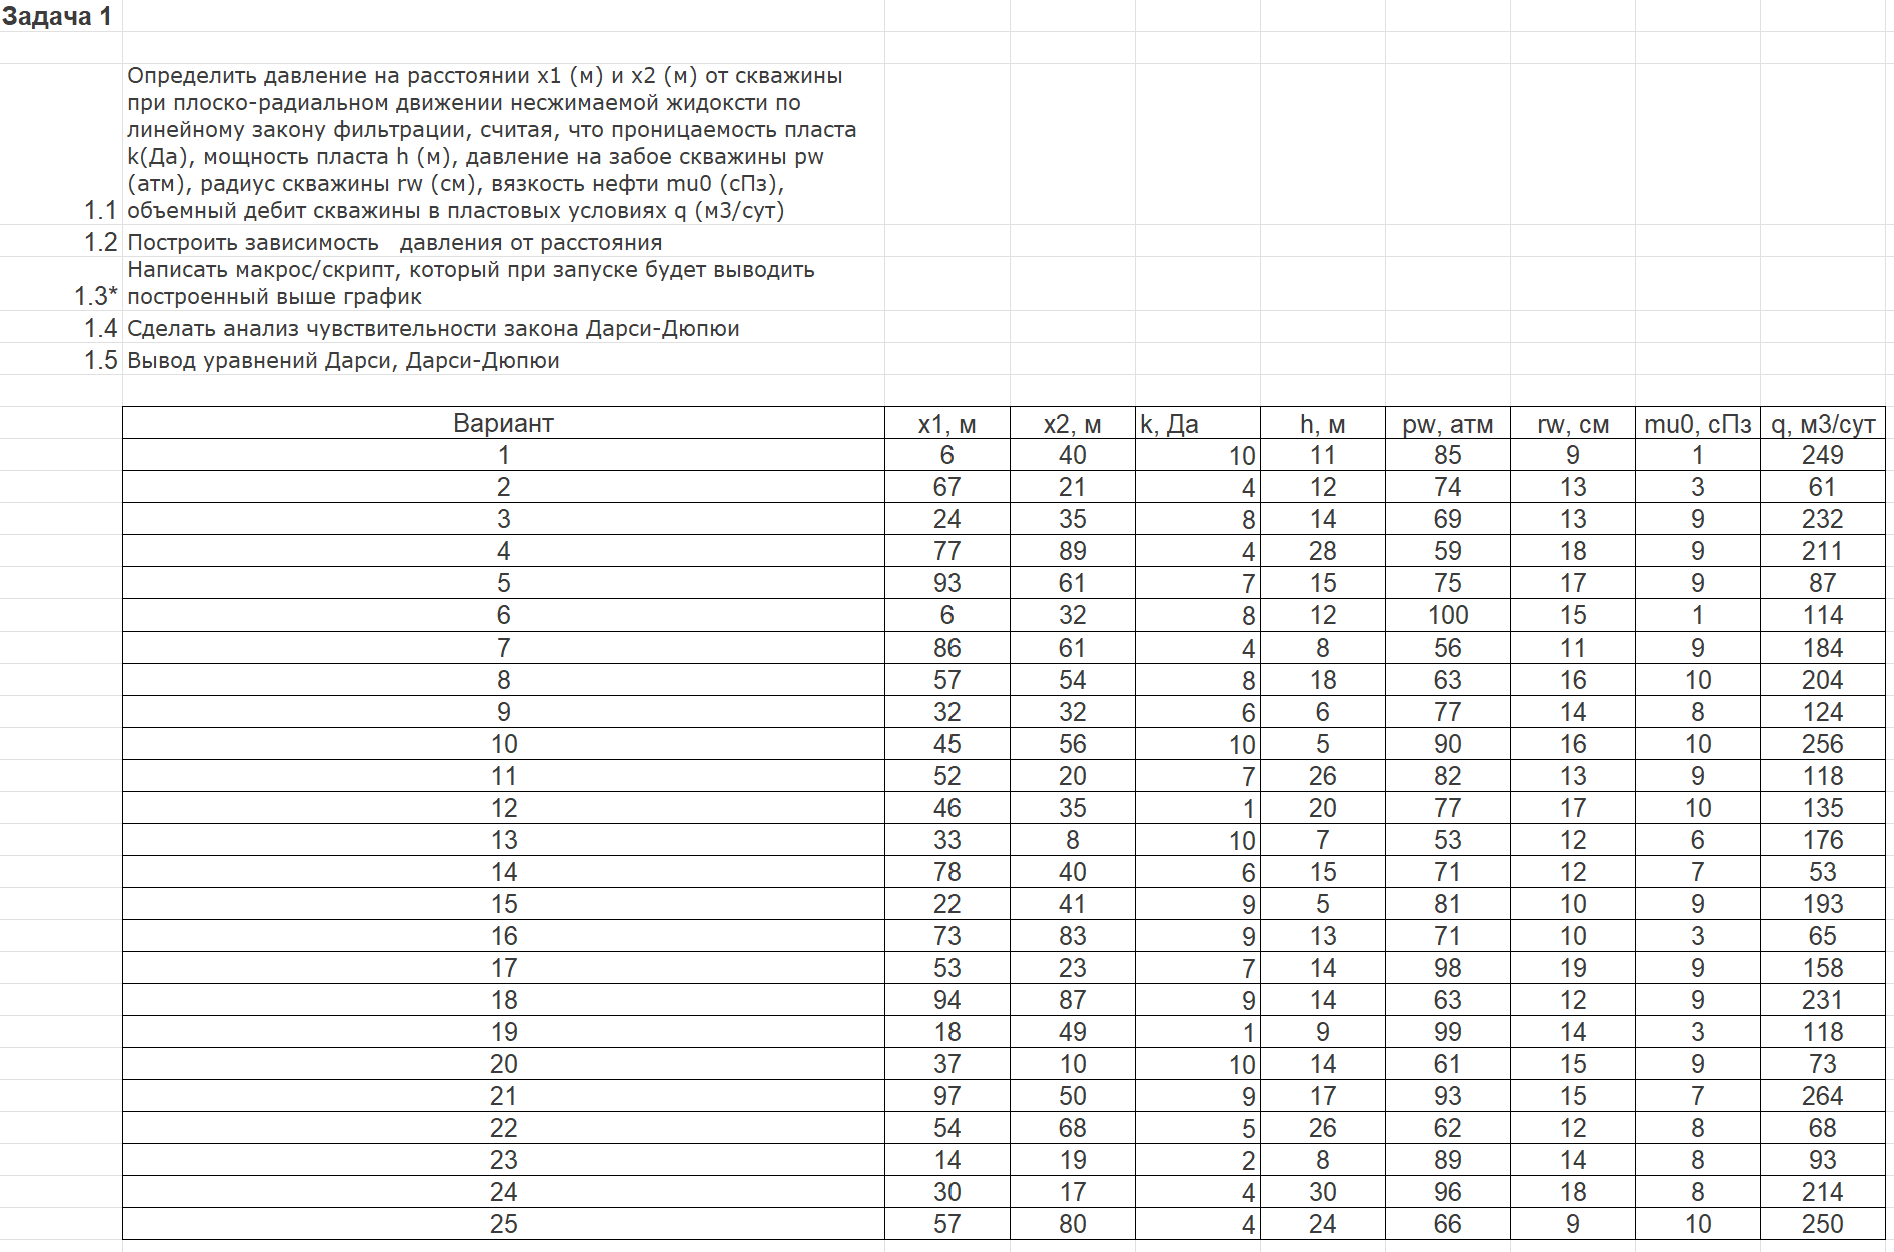
\includegraphics[width=\textwidth]{task1}


\subsection{Расчёт давления по формуле Дюпюи}

Давление на расстоянии $x_1$:
\begin{multline}
P_{x_1}=P_w+\frac{18.41\cdot Q\mu}{kh}\left(\ln{\left(\frac{x_1}{r_w}\right)+S}\right)
=\\=71\text{ атм}+\frac{18.41\cdot 65\dfrac{\text{м}^3}{\text{сут}}\cdot3\text{ сПз}}{9000\text{ мД}\cdot 13\text{ м}}\left(\ln{\left(\frac{73\text{ м}}{0,1\text{ м}}\right)}+0\right)\approx 71.2023\text{ атм}
\end{multline}

Давление на расстоянии $x_2$:
\begin{multline}
P_{x_1}=P_w+\frac{18.41\cdot Q\mu}{kh}\left(\ln{\left(\frac{x_2}{r_w}\right)+S}\right)
=\\=71\text{ атм}+\frac{18.41\cdot 65\dfrac{\text{м}^3}{\text{сут}}\cdot3\text{ сПз}}{9000\text{ мД}\cdot 13\text{ м}}\left(\ln{\left(\frac{83\text{ м}}{0,1\text{ м}}\right)}+0\right)\approx 71.2062\text{ атм}
\end{multline}


\subsection{График зависимости давления от расстояния}

\subsection{Код для вывода графика}

\subsection{Анализ чувствительности формулы Дюпюи}

Вид формулы Дюпюи на установившемся режиме в промысловых единицах со скин-фактором:

\beq
Q=\frac{kh}{18.41\cdot\mu}\,\frac{P_e-P_w}{\ln{\left(\dfrac{r_e}{r_w}\right)+S}}
\eeq

Jupyter-тетрадь с кодом для построения графика и проведения анализа чувствительности доступна по ссылке: \href{https://colab.research.google.com/github/mualal/notebooks-source/blob/master/6_pressure.ipynb}{OPEN IN COLAB}.

\subsection{Вывод уравнения Дарси и формулы Дюпюи}

Приравнивая значение потоковой скорости, найденное из геометрии пласта, к значению, найденному из закона Дарси, получим дифференциальное уравнение притока флюида к скважине.

Дюпюи составил и решил это дифференциальное уравнение для случая границы в виде цилиндрической области (для радиального режима течения).

\beq
\frac{Q}{A}=\frac{k}{\mu}\frac{dP}{dx}\Rightarrow\frac{Q}{2\pi h}\int\limits_{r_w}^{r_e}{\frac{dr}{r}}=\frac{k}{\mu}\int\limits_{P_w}^{P_e}{dp}\Rightarrow Q=\frac{2\pi kh}{\mu}\frac{P_e-P_w}{\ln{\left(\dfrac{r_e}{r_w}\right)}}
\eeq

Формула получена в СИ.
При пересчёте в промысловые единицы измерения формула Дюпюи примет следующий вид:

\beq
Q=\frac{kh}{18.41\cdot\mu}\,\frac{P_e-P_w}{\ln{\left(\dfrac{r_e}{r_w}\right)}}
\eeq

\section{Задание 2 от 14.09.2022}
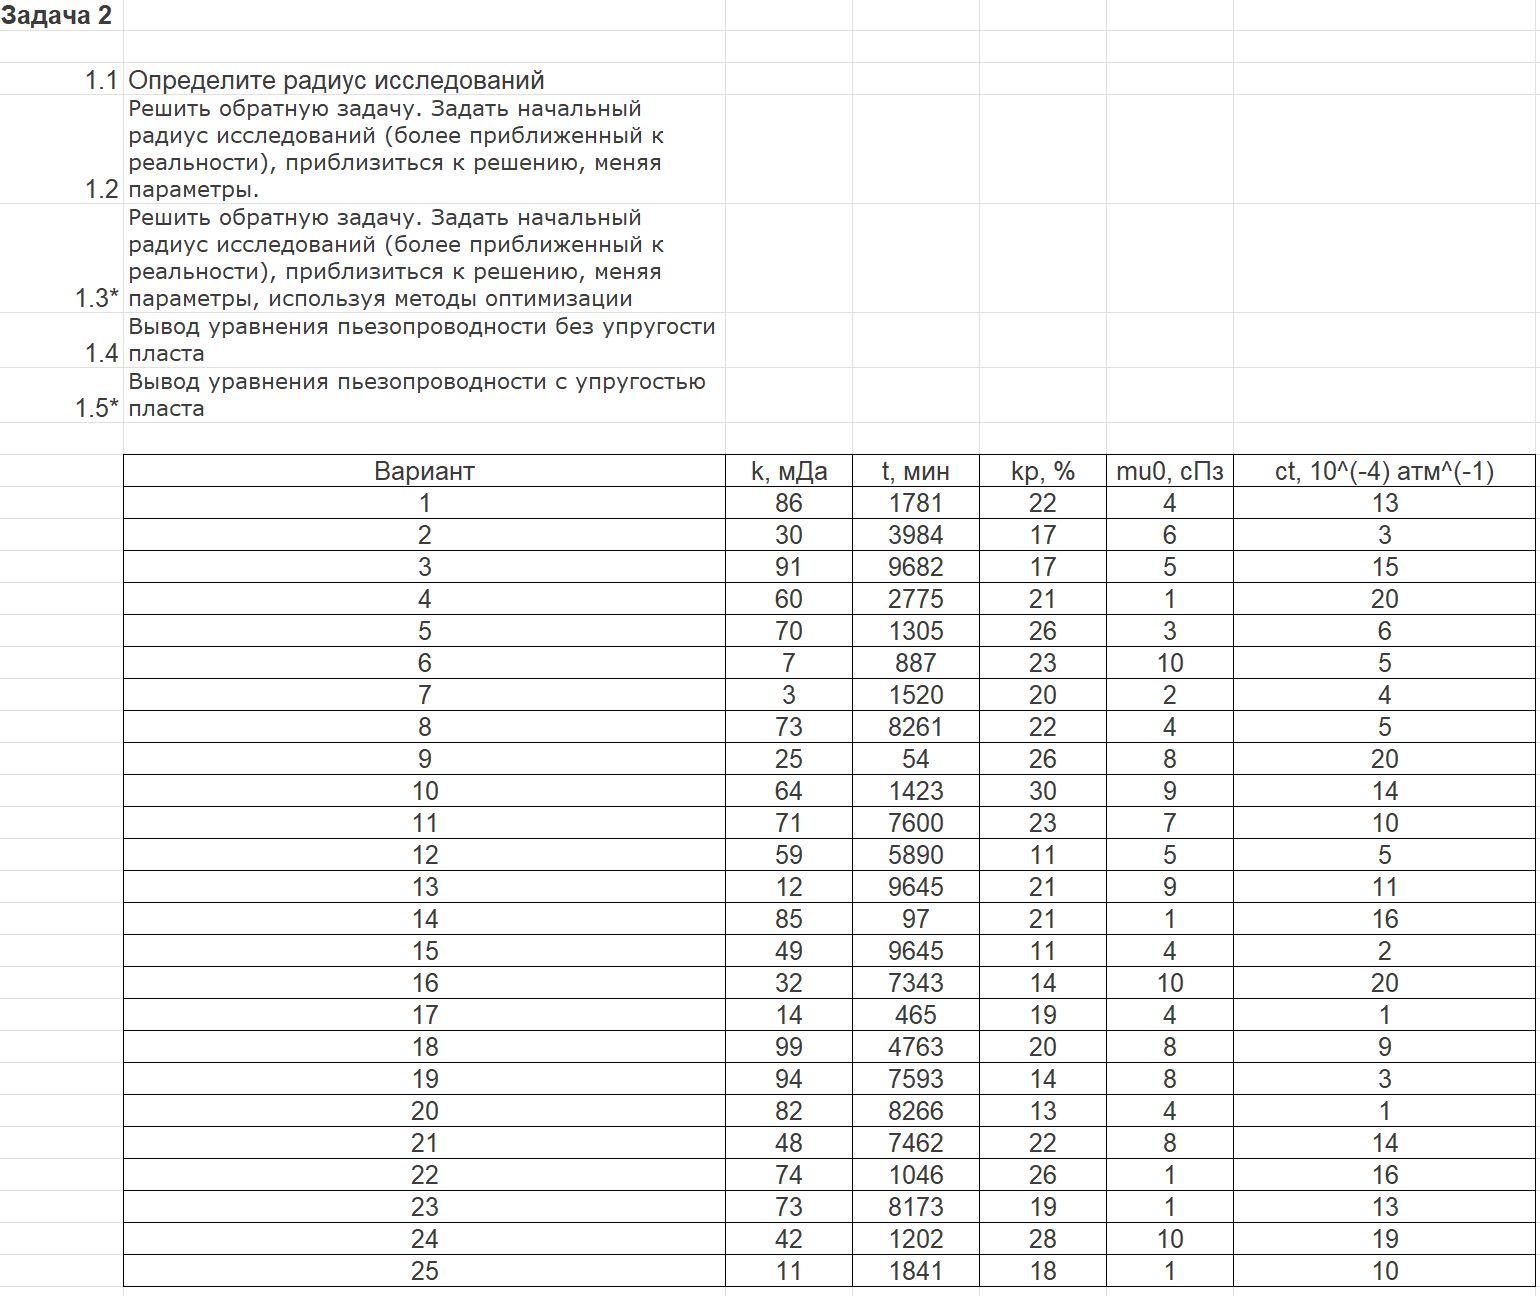
\includegraphics[width=\textwidth]{task2}

\subsection{Радиус исследований}

\beq
r_{inv}=0.037\sqrt{\frac{kt}{\varphi \mu c_t}}=0.037\sqrt{\frac{32\text{ мДа}\cdot 7343\text{ мин}}{0.14\cdot 10\text{ сПз}\cdot 20\cdot 10^{-4}\dfrac{\text{1}}{\text{атм}}}}\approx 338.95\text{ м}
\eeq

График зависимости радиуса исследования от произведения проницаемости и времени построен по ссылке: \href{https://colab.research.google.com/github/mualal/notebooks-source/blob/master/7_exploration_radius.ipynb}{OPEN IN COLAB}.

\subsection{Решение обратной задачи}

Зададим радиус исследования $r_{inv}=100\text{ м}$, тогда:

\beq
kt=\varphi\mu c_t\left(\dfrac{r_{inv}}{0.037}\right)^2=0.14\cdot 10\text{ сПз}\cdot 20\cdot 10^{-4}\frac{1}{\text{атм}}\cdot \left(\frac{100\text{ м}}{0.037}\right)^{\!2}\approx 20452.89\text{ мДа}\cdot\text{мин}
\eeq

При проницаемости $k=32\text{ мДа}$, время исследования будет составлять:

\beq
t\approx\frac{20452.89\text{ мДа}\cdot\text{мин}}{32\text{ мДа}}\approx 639 \text{ мин}\approx10.65\text{ ч}.
\eeq

\subsection{Вывод уравнения пьезопроводности без упругости пласта}

1) Набор уравнений:
\begin{itemize}
	\item неразрывность потока
	\beq\label{Continuity}
	\frac{\partial\left(\rho_f\varphi\right)}{\partial t}+\pmb{\nabla}\cdot\left(\rho_f\varphi \pmb{v_f}\right)=q_f(\pmb{x})
	\eeq
	\item закон Дарси
	\beq\label{Darcy}
	\pmb{W}=-\frac{k}{\mu_f}\cdot\pmb{\nabla} p
	\eeq
	\item сжимаемость флюида
	\beq\label{Compressibility}
	p-p_0=K_f\frac{\rho_f-\rho_f^0}{\rho_f^0}
	\eeq
\end{itemize}

На этих уравнениях строится основное уравнение гидродинамики пласта -- уравнение пьезопроводности.

2) Насыщенности и относительные фазовые проницаемости (для нескольких флюидов)

3) Геометрия (сложное строение пласта)

\subsubsection{В векторной форме (быстрый, но не совсем строгий вывод)}

В предположении неподвижности скелета ($\pmb{v_s}\approx \pmb{0}$ и $\varphi(t)=\textrm{const}$) верно равенство $\pmb{W}\approx\varphi \pmb{v_f}$. Подставляя в закон Дарси \eqref{Darcy}, получаем:
\beq\label{DarcyWithSkeletNotMoving}
\varphi \pmb{v_f}=-\frac{k}{\mu_f}\cdot\pmb{\nabla} p
\eeq

Условие сжимаемости флюида \eqref{Compressibility} перепишем в дифференциальной форме:
\beq\label{CompressibilityDiff}
\frac{\partial p}{\partial t}=\frac{K_f}{\rho_f^0}\frac{\partial\rho_f}{\partial t}
\eeq

Учитывая предположение о неподвижности скелета, перепишем уравнение неразрывности потока:
\beq\label{ContinuityWithSkeletNotMoving}
\varphi\frac{\partial\rho_f}{\partial t}+\pmb{\nabla}\cdot\left(\rho_f\varphi\pmb{v_f}\right)=q_f(\pmb{x})
\eeq

Подставляя \eqref{DarcyWithSkeletNotMoving} и \eqref{CompressibilityDiff} в \eqref{ContinuityWithSkeletNotMoving}, при отсутствии источникового слагаемого ($q_f(\pmb{x})=0$) получаем:
\beq
\varphi\frac{\rho_f^0}{K_f}\frac{\partial p}{\partial t}-\pmb{\nabla}\cdot\left(\rho_f\frac{k}{\mu_f}\pmb{\nabla} p\right)=0
\eeq

При дополнительном условии слабосжимаемости флюида ($\rho_f\approx\rho_f^0=\textrm{const}$) получаем:
\beq
\frac{\partial p}{\partial t}=\frac{kK_f}{\mu_f\varphi}\pmb{\nabla}^2p
\eeq

Это уравнение пьезопроводности (без упругости пласта), полученное в приближении слабосжимаемого флюида, неподвижного и недеформируемого пласта.

\subsubsection{В покомпонентной форме с обезразмериванием (от Шеля Е.В.)}

Запишем ЗСМ для флюида:
\beq
\frac{\partial r_f}{\partial t}+\partial_i\left(r_f v_i^f\right)=0
\eeq

Закон Дарси в "<школьной"> форме:
\beq
Q=-\frac{\Delta p}{L}\frac{k}{\mu}S
\eeq

Закон Дарси в дифференциальной форме:
\beq\label{DarcyDiffShel}
W_i=-\frac{k_{ij}}{\mu}\partial_j p,
\eeq
где $W_i=\varphi v_i^f$ -- потоковая относительная скорость флюида.

Учитывая связь эффективной и истинной плотностей ($r_f=\varphi\rho_f$), перепишем ЗСМ для флюида:
\beq\label{ContinuityShel}
\frac{\partial\left(\rho_f\varphi\right)}{\partial t}+\partial_i\left(\rho_f\varphi v_i^f\right)=0
\eeq

Подставляя \eqref{DarcyDiffShel} в \eqref{ContinuityShel}, получаем:
\beq\label{GeneralPiezo}
\frac{\partial\left(\rho_f\varphi\right)}{\partial t}-\partial_i\left(\rho_f\frac{k_{ij}}{\mu}\partial_j p\right)=0
\eeq

--------------------------------------------------------------------

Замыкающее соотношение (связь плотности флюида и давления):
\beq\label{Zam1}
\rho_f=\rho_f^0\left(1+c_f\left(p-p_0\right)\right),
\eeq
где $c_f$ -- сжимаемость флюида (1/Па).


Замыкающее соотношение (связь пористости и давления):
\beq\label{Zam2}
\varphi=\varphi^0+c_{\text{п}}\left(p-p_0\right),
\eeq
где $c_{\text{п}}$ -- сжимаемость пор (не равно сжимаемости породы).

--------------------------------------------------------------------

Продифференцируем по времени замыкающее соотношение \eqref{Zam1}:
\beq\label{DiffZam1}
\frac{\partial\rho_f}{\partial t}=c_f\rho_f^0\frac{\partial p}{\partial t}
\eeq

Продифференцируем по пространству замыкающее соотношение \eqref{Zam1}:
\beq\label{GradZam1}
\partial_i\rho_f=c_f\rho_f^0\partial_i p
\eeq

Продифференцируем по времени замыкающее соотношение \eqref{Zam2}:
\beq\label{DiffZam2}
\frac{\partial\varphi}{\partial t}=c_\text{п}\frac{\partial p}{\partial t}
\eeq

Продифференцируем по пространству замыкающее соотношение \eqref{Zam2}:
\beq\label{GradZam2}
\partial_i\varphi=c_\text{п}\partial_i p
\eeq

--------------------------------------------------------------------

Раскрывая производные произведений в \eqref{GeneralPiezo}, получаем:
\beq\label{OpenGeneralContinuity}
\frac{\partial\rho_f}{\partial t}\varphi+\rho_f\frac{\partial\varphi}{\partial t}-\frac{k_{ij}}{\mu}\partial_j p\,\partial_i\rho_f-\rho_f\partial_j p\,\partial_i\!\left(\frac{k_{ij}}{\mu}\right)-\rho_f\frac{k_{ij}}{\mu}\left(\partial_i\partial_j p\right)=0
\eeq

Подставляя \eqref{DiffZam1}, \eqref{GradZam1}, \eqref{DiffZam2} и \eqref{GradZam2} в \eqref{OpenGeneralContinuity}, получаем:
\begin{multline}\label{Expanded}
c_f\rho_f^0\frac{\partial p}{\partial t}\varphi+\rho_f c_\text{п}\frac{\partial p}{\partial t}-\frac{k_{ij}}{\mu}\partial_j p\,c_f\rho_f^0\,\partial_i p-\frac{\rho_f}{\mu}\partial_j p\,\partial_i k_{ij}+\\+\rho_f\,\partial_j p\,k_{ij}\frac{\partial\mu}{\partial p}\frac{1}{\mu^2}\partial_i p-\rho_f\frac{k_{ij}}{\mu}\left(\partial_i\partial_j p\right)=0
\end{multline}

--------------------------------------------------------------------

Перед анализом физических уравнений всегда делают масштабный анализ, чтобы понять, какие слагаемые в уравнении важны, а какие не важны (пример: уравнение Навье-Стокса с числами Струхаля, Эйлера, Рейнольдса, Фруда).

Спойлер: ГДМ симуляторы не решают уравнение пьезопроводности в классическом виде, а решают закон сохранения массы, в который они подставляют закон Дарси.

Далее необходимо выделить характерные масштабные факторы, обезразмерив каждую из функций в уравнении.

Введём безразмерное давление $\tilde{p}$ такое, что:
\beq
p=\tilde{p}\cdot p_0,
\eeq
где $p_0$ -- пластовое давление.

Введём безразмерное расстояние $\tilde{r}$ такое, что:
\beq
\vec{r}=\tilde{r}\cdot L,
\eeq
где $L$ -- некое характерное расстояние (например, между скважинами).

Введём безразмерную проницаемость $\tilde{k}_{ij}$ такую, что:
\beq
k_{ij}=\tilde{k}_{ij}\cdot k_0,
\eeq
где $k_0$ -- некая характерная проницаемость.

Введём безразмерную вязкость $\tilde{\mu}$ такую, что:
\beq
\mu=\tilde{\mu}\cdot\mu_0,
\eeq
где $\mu_0$ -- некая характерная вязкость.

Все безразмерные функции (с волной) порядка единицы.

--------------------------------------------------------------------

Перепишем \eqref{Expanded} в введённых безразмерных величинах, разделив обе части этого уравнения на $\rho_f^0$:
\begin{multline}
\frac{\partial p}{\partial t}\left(\varphi c_f+\frac{\rho_f}{\rho_f^0}\cdot c_\text{п}\right)-\frac{k_0}{\mu_0}\frac{p_0^2}{L^2}c_f\frac{\tilde{k}_{ij}}{\tilde{\mu}}\,\tilde{\partial}_i\tilde{p}\,\tilde{\partial}_j\tilde{p}-\frac{\rho_f}{\rho_f^0}\frac{k_0\,p_0}{\mu_0L^2}\frac{\tilde{k}_{ij}}{\tilde{\mu}}\,\tilde{\partial}_j\tilde{p}\,\tilde{\partial}_i\tilde{k}_{ij}+\\+\frac{\rho_f}{\rho_f^0}\frac{p_0\,k_0}{L^2\mu_0}\,\tilde{\partial}_j\tilde{p}\,\tilde{k}_{ij}\frac{\partial\tilde{\mu}}{\partial\tilde{p}}\frac{1}{\tilde{\mu}^2}\,\tilde{\partial}_i\tilde{p}-\frac{\rho_f}{\rho_f^0}\frac{k_0}{\mu_0}\frac{p_0}{L^2}\,\frac{\tilde{k}_{ij}}{\tilde{\mu}}\left(\tilde{\partial}_i\tilde{\partial}_j\tilde{p}\right)=0
\end{multline}

Вынесли все масштабные множители. Далее делим обе части уравнения на множитель перед старшей производной $\left(\text{на }\frac{k_0\,p_0}{\mu_0\,L^2}\right)$, т.е. обезразмериваем уравнение:
\begin{multline}\label{PiezoEqDiv}
\frac{\mu_0L^2}{k_0p_0}\cdot\frac{\partial p}{\partial t}\left(\varphi c_f+\frac{\rho_f}{\rho_f^0}\cdot c_\text{п}\right)-p_0c_f\frac{\tilde{k}_{ij}}{\tilde{\mu}}\,\tilde{\partial}_i\tilde{p}\,\tilde{\partial}_j\tilde{p}-\frac{\rho_f}{\rho_f^0}\frac{\tilde{k}_{ij}}{\tilde{\mu}}\,\tilde{\partial}_j\tilde{p}\,\tilde{\partial}_i\tilde{k}_{ij}+\\+\frac{\rho_f}{\rho_f^0}\frac{\partial\tilde{\mu}}{\partial\tilde{p}}\frac{1}{\tilde{\mu}^2}\tilde{k}_{ij}\,\tilde{\partial}_j\tilde{p}\,\tilde{\partial}_i\tilde{p}-\frac{\rho_f}{\rho_f^0}\frac{\tilde{k}_{ij}}{\tilde{\mu}}\left(\tilde{\partial}_i\tilde{\partial}_j\tilde{p}\right)=0
\end{multline}

--------------------------------------------------------------------

Сделаем 3 важных приближения:
\begin{enumerate}
	\item $p_0 c_f\ll 1$ (прикинем: сжимаемость воды порядка $10^{-5}\text{ атм}^{-1}=10^{-10}\text{ Па}^{-1}$; характерные значения давлений на глубинах, равных нескольким километрам, составляют сотни атмосфер; таким образом, произведение порядка $10^{-3}$, что много меньше единицы; но такое приближение не работает для газа: для него рассматриваемое произведение порядка единицы); это приближение фактически равносильно приближению $\rho_f\approx\rho_f^0$;
	\item $\tilde{\partial}_i\tilde{k}_{ij}\ll 1$ (считаем, что на характерном масштабе задачи по данному направлению проницаемость изменяется незначительно, не больше 10 процентов);
	\item $\dfrac{\partial\tilde{\mu}}{\partial\tilde{p}}\ll 1$ (считаем, что отмасштабированный график проницаемости от давления пологий -- этот факт подтверждается экспериментально -- вязкость слабо зависит от давления)
\end{enumerate}

Тогда уравнение \eqref{PiezoEqDiv} перепишется в следующем виде (убрали слагаемые с пренебрежимо малыми множителями в рамках сделанных приближений и вернулись от безразмерных функций с волной к обычным функциям):
\beq
\frac{\partial p}{\partial t}\underbrace{\left(\varphi c_f+c_\text{п}\right)}_{c_t}-\frac{k_{ij}}{\mu}\partial_i\partial_j p=0
\eeq
(заметим, что если есть анизотропия проницаемости, то лапласиана в уравнении не будет).

Получаем классическое уравнение пьезопроводности:
\beq
\frac{\partial p}{\partial t}-\frac{k_{ij}}{\mu c_t}\partial_i\partial_j p=0,
\eeq
где $c_t$ -- это полная сжимаемость.

Замечание. Но есть литература, в которой $c_t=c_f+\frac{c_\text{п}}{\varphi}$, тогда уравнение пьезопроводности будет выглядеть так:
\beq
\frac{\partial p}{\partial t}-\frac{k_{ij}}{\mu\varphi c_t}\partial_i\partial_j p=0
\eeq

--------------------------------------------------------------------

Пусть тензор проницаемости изотропен $k_{ij}=k_0\cdot\delta_{ij}$, тогда:
\beq
\frac{\partial p}{\partial t}-\frac{k_0}{\mu c_t}\delta_{ij}\,\partial_i\partial_j p=0\Leftrightarrow\frac{\partial p}{\partial t}-\frac{k_0}{\mu c_t}\Delta p=0
\eeq
(получили всем известный вид уравнения пьезопроводности).


\subsection{Вывод уравнения пьезопроводности с упругостью пласта}

Задача со звёздочкой. Ещё думаю.

\section{Задание от 21.09.2022}

Jupyter-тетрадь с кодом обработки ОФП доступна по ссылке: \href{https://github.com/mualal/notebooks-source/blob/master/9_labdata_relative_permeabilities.ipynb}{OPEN IN COLAB}.

\section{Задание от 28.09.2022}

\section{Задание от 05.10.2022}

\end{document}
